\chapter*{Resultados}\label{ch:resultados}
\addcontentsline{toc}{chapter}{Capitulo 6. Resultados}

\section*{}
\addtocounter{section}{1}
\setcounter{subsection}{0}

En esta sección, se presentan los resultados obtenidos de los experimentos realizados. Los mismos se presentan en distintas tablas que se pueden dividir en dos grandes grupos: i) Análisis del método propuesto y; ii) Análisis del método propuesto y algoritmos del estado del arte. Las matrices de confusión calculadas para generar las matrices de confusión promedio utilizadas en este apartado, se encuentran en la Tabla \ref{tab:anexo-confusion}, ubicada en el anexo de este trabajo.

\subsection{Análisis del método propuesto}

A continuación se muestran distintas ejecuciones del método EQuAL, de forma de generar resultados estadísticamente significativos, como se explicó en el apartado 5.6 (Método de validación). Se presentan tablas correspondientes a un tamaño de muestra en particular: 100, 500, 1000, 1500 y 2000 pares de preguntas; y en cada una de ellas, las filas corresponden a un número de clusters \(k\) distinto. Además, en todas las ejecuciones se realizaron 100 ejecuciones de clustering, es decir, teniendo en cuenta que se ensamblaron 5 algoritmos del estado del arte, cada una de las ejecuciones de un valor \(k\) en particular, se realizaron un total de \(500\) ejecuciones de clustering. Como método de evaluación del rendimiento de método EQuAL, se utilizan matrices de confusión. En la tabla, se muestran, por cada fila, una matriz de confusión promedio de cada una de las 10 ejecuciones para ese tamaño de muestra y número de clusters k. Como indicador de rendimiento final, se suman las columnas “\% 0/0” y “\% 1/1” para obtener la precisión, y el error es derivado de \(1 - precisi\acute{o}n\) o sumando “\% 0/1” y “\% 1/0”. Para finalizar, se resalta el mejor resultado correspondiente a un valor k para cada tamaño de muestra.

\begin{table}[]
	\centering
	\begin{tabular}{|c|c|c|c|c|c|c|}
		\hline
		\rowcolor[HTML]{CFE2F3}
		\textbf{Número de Clusters (k)} & \textbf{\% 0/0} & \textbf{\% 0/1} & \textbf{\% 1/0} & \textbf{\% 1/1} & \textbf{Precisión} & \textbf{Error} \\ \hline
		5  & 0.475 & 0.119 & 0.203 & 0.203 & 0.678 & 0.322 \\ \hline
		10 & 0.491 & 0.103 & 0.215 & 0.191 & 0.682 & 0.318 \\ \hline
		15 & 0.444 & 0.15  & 0.164 & 0.242 & 0.686 & 0.314 \\ \hline
		20 & 0.449 & 0.145 & 0.173 & 0.233 & 0.682 & 0.318 \\ \hline
		25 & 0.435 & 0.159 & 0.15  & 0.256 & 0.691 & 0.309 \\ \hline
		\rowcolor[HTML]{D9EAD3}
		30 & 0.435 & 0.159 & 0.145 & 0.261 & 0.696 & 0.304 \\ \hline
		35 & 0.444 & 0.15  & 0.157 & 0.249 & 0.693 & 0.307 \\ \hline
		40 & 0.408 & 0.186 & 0.123 & 0.283 & 0.691 & 0.309 \\ \hline
		45 & 0.459 & 0.135 & 0.176 & 0.23  & 0.689 & 0.311 \\ \hline
		50 & 0.463 & 0.131 & 0.177 & 0.229 & 0.692 & 0.308 \\ \hline
	\end{tabular}
	\caption{Matrices de confusión promedio del método EQuAL. 100 muestras de 100 pares de preguntas cada una. }
	\label{tab:analisis-100-100}
\end{table}

\begin{table}[]
	\centering
	\begin{tabular}{|c|c|c|c|c|c|c|}
		\hline
		\rowcolor[HTML]{CFE2F3}
		\textbf{Número de Clusters (k)} & \textbf{\% 0/0} & \textbf{\% 0/1} & \textbf{\% 1/0} & \textbf{\% 1/1} & \textbf{Precisión} & \textbf{Error} \\ \hline
		5  & 0.4562 & 0.1458 & 0.1908 & 0.2072 & 0.6634 & 0.3366 \\ \hline
		10 & 0.4468 & 0.1596 & 0.1658 & 0.2278 & 0.6746 & 0.3254 \\ \hline
		15 & 0.4356 & 0.1708 & 0.1542 & 0.2394 & 0.675  & 0.325  \\ \hline
		20 & 0.4316 & 0.1748 & 0.1444 & 0.2492 & 0.6808 & 0.3192 \\ \hline
		25 & 0.4306 & 0.1758 & 0.1468 & 0.2468 & 0.6774 & 0.3226 \\ \hline
		30 & 0.4322 & 0.1742 & 0.1476 & 0.246  & 0.6782 & 0.3218 \\ \hline
		35 & 0.4334 & 0.173  & 0.1458 & 0.2478 & 0.6812 & 0.3188 \\ \hline
		40 & 0.4272 & 0.1792 & 0.1378 & 0.2558 & 0.683  & 0.317  \\ \hline
		45 & 0.439  & 0.1674 & 0.1488 & 0.2448 & 0.6838 & 0.3162 \\ \hline
		\rowcolor[HTML]{D9EAD3}
		50 & 0.4378 & 0.1686 & 0.1454 & 0.2482 & 0.686  & 0.314  \\ \hline
	\end{tabular}
	\caption{Matrices de confusión promedio del método EQuAL. 100 muestras de 500 pares de preguntas cada una. }
	\label{tab:analisis-100-500}
\end{table}

\begin{table}[]
	\centering
	\begin{tabular}{|c|c|c|c|c|c|c|}
		\hline
		\rowcolor[HTML]{CFE2F3}
		\textbf{Número de Clusters (k)} & \textbf{\% 0/0} & \textbf{\% 0/1} & \textbf{\% 1/0} & \textbf{\% 1/1} & \textbf{Precisión} & \textbf{Error} \\ \hline
		5  & 0.4488 & 0.1561 & 0.1902 & 0.2049 & 0.6537 & 0.3463 \\ \hline
		10 & 0.4482 & 0.1559 & 0.1847 & 0.2112 & 0.6594 & 0.3406 \\ \hline
		15 & 0.4502 & 0.1539 & 0.188  & 0.2079 & 0.6581 & 0.3419 \\ \hline
		20 & 0.4655 & 0.1386 & 0.2007 & 0.1952 & 0.6607 & 0.3393 \\ \hline
		25 & 0.462  & 0.1421 & 0.1957 & 0.2002 & 0.6622 & 0.3378 \\ \hline
		30 & 0.461  & 0.1431 & 0.1933 & 0.2026 & 0.6636 & 0.3364 \\ \hline
		35 & 0.4608 & 0.1433 & 0.1933 & 0.2026 & 0.6634 & 0.3366 \\ \hline
		40 & 0.466  & 0.1381 & 0.2016 & 0.1943 & 0.6603 & 0.3397 \\ \hline
		45 & 0.4445 & 0.1596 & 0.1765 & 0.2194 & 0.6639 & 0.3361 \\ \hline
		\rowcolor[HTML]{D9EAD3}
		50 & 0.4521 & 0.152  & 0.1804 & 0.2155 & 0.6676 & 0.3324 \\ \hline
	\end{tabular}
	\caption{Matrices de confusión promedio del método EQuAL. 100 muestras de 1000 pares de preguntas cada una. }
	\label{tab:analisis-100-1000}
\end{table}

\begin{table}[]
	\centering
	\begin{tabular}{|c|c|c|c|c|c|c|}
		\hline
		\rowcolor[HTML]{CFE2F3}
		\textbf{Número de Clusters (k)} & \textbf{\% 0/0} & \textbf{\% 0/1} & \textbf{\% 1/0} & \textbf{\% 1/1} & \textbf{Precisión} & \textbf{Error} \\ \hline
		5  & 0.4297 & 0.1773 & 0.1713 & 0.2217 & 0.6514 & 0.3486 \\ \hline
		10 & 0.4709 & 0.136  & 0.2035 & 0.1896 & 0.6605 & 0.3395 \\ \hline
		15 & 0.4293 & 0.1777 & 0.1633 & 0.2297 & 0.659  & 0.341  \\ \hline
		20 & 0.4269 & 0.18   & 0.1624 & 0.2307 & 0.6576 & 0.3424 \\ \hline
		25 & 0.4383 & 0.1687 & 0.171  & 0.222  & 0.6603 & 0.3397 \\ \hline
		30 & 0.4509 & 0.156  & 0.1824 & 0.2107 & 0.6616 & 0.3384 \\ \hline
		35 & 0.4599 & 0.1471 & 0.1893 & 0.2037 & 0.6636 & 0.3364 \\ \hline
		40 & 0.4439 & 0.1631 & 0.1753 & 0.2177 & 0.6616 & 0.3384 \\ \hline
		45 & 0.4485 & 0.1585 & 0.1765 & 0.2165 & 0.665  & 0.335  \\ \hline
		\rowcolor[HTML]{D9EAD3}
		50 & 0.451  & 0.156  & 0.1733 & 0.2197 & 0.6707 & 0.3293 \\ \hline
	\end{tabular}
	\caption{Matrices de confusión promedio del método EQuAL. 100 muestras de 1500 pares de preguntas cada una. }
	\label{tab:analisis-100-1500}
\end{table}

\begin{table}[]
	\centering
	\begin{tabular}{|c|c|c|c|c|c|c|}
		\hline
		\rowcolor[HTML]{CFE2F3}
		\textbf{Número de Clusters (k)} & \textbf{\% 0/0} & \textbf{\% 0/1} & \textbf{\% 1/0} & \textbf{\% 1/1} & \textbf{Precisión} & \textbf{Error} \\ \hline
		5  & 0.4409 & 0.1668 & 0.1739 & 0.2184 & 0.6593 & 0.3407 \\ \hline
		10 & 0.4496 & 0.1581 & 0.1808 & 0.2115 & 0.6611 & 0.3389 \\ \hline
		15 & 0.446  & 0.1617 & 0.1737 & 0.2186 & 0.6646 & 0.3354 \\ \hline
		20 & 0.4476 & 0.1601 & 0.1774 & 0.2149 & 0.6625 & 0.3375 \\ \hline
		25 & 0.4637 & 0.144  & 0.1914 & 0.2009 & 0.6646 & 0.3354 \\ \hline
		30 & 0.431  & 0.1767 & 0.1586 & 0.2337 & 0.6647 & 0.3353 \\ \hline
		35 & 0.4451 & 0.1626 & 0.1689 & 0.2234 & 0.6685 & 0.3315 \\ \hline
		40 & 0.4569 & 0.1508 & 0.1788 & 0.2135 & 0.6704 & 0.3296 \\ \hline
		45 & 0.428  & 0.1797 & 0.152  & 0.2403 & 0.6683 & 0.3317 \\ \hline
		\rowcolor[HTML]{D9EAD3}
		50 & 0.449  & 0.1587 & 0.1719 & 0.2204 & 0.6694 & 0.3306 \\ \hline
	\end{tabular}
	\caption{Matrices de confusión promedio del método EQuAL. 100 muestras de 2000 pares de preguntas cada una. }
	\label{tab:analisis-100-2000}
\end{table}

\begin{table}[]
	\centering
	\footnotesize
	\begin{tabular}{|
			>{\columncolor[HTML]{FFE599}}c |c|c|c|c|c|c|c|}
		\hline
		\tiny\textbf{\begin{tabular}[c]{@{}c@{}}k / \\ Tam. de muestra\end{tabular}} &
		\cellcolor[HTML]{FFE599}\textbf{100} &
		\cellcolor[HTML]{FFE599}\textbf{500} &
		\cellcolor[HTML]{FFE599}\textbf{1000} &
		\cellcolor[HTML]{FFE599}\textbf{1500} &
		\cellcolor[HTML]{FFE599}\textbf{2000} &
		\cellcolor[HTML]{FFE599}\textbf{Media} &
		\cellcolor[HTML]{FFE599}\textbf{Varianza} \\ \hline
		\textbf{5}  & 0.322 & 0.3366 & 0.3463 & 0.3486 & 0.3407 & 0.33884                         & 0.000442972                                                \\ \hline
		\textbf{10} & 0.318 & 0.3254 & 0.3406 & 0.3395 & 0.3389 & 0.33248                         & \cellcolor[HTML]{D9EAD3}{\color[HTML]{333333} 0.000416228} \\ \hline
		\textbf{15} & 0.314 & 0.325  & 0.3419 & 0.341  & 0.3354 & 0.33146                         & 0.000562112                                                \\ \hline
		\textbf{20} & 0.318 & 0.3192 & 0.3393 & 0.3424 & 0.3375 & 0.33128                         & 0.000548948                                                \\ \hline
		\textbf{25} & 0.309 & 0.3226 & 0.3378 & 0.3397 & 0.3354 & 0.3289                          & 0.0006738                                                  \\ \hline
		\textbf{30} & 0.304 & 0.3218 & 0.3364 & 0.3384 & 0.3353 & 0.32718                         & 0.000843088                                                \\ \hline
		\textbf{35} & 0.307 & 0.3188 & 0.3366 & 0.3364 & 0.3315 & 0.32606                         & 0.000663592                                                \\ \hline
		\textbf{40} & 0.309 & 0.317  & 0.3397 & 0.3384 & 0.3296 & 0.32674                         & 0.000721672                                                \\ \hline
		\textbf{45} & 0.311 & 0.3162 & 0.3361 & 0.335  & 0.3317 & 0.326                           & 0.00053654                                                 \\ \hline
		\textbf{50} & 0.308 & 0.314  & 0.3324 & 0.3293 & 0.3306 & \cellcolor[HTML]{D9EAD3}0.32286 & 0.000491712                                                \\ \hline
		\textbf{Media} &
		\cellcolor[HTML]{D9EAD3}0.312 &
		0.32166 &
		0.33871 &
		0.33887 &
		0.33466 &
		\multicolumn{1}{l|}{\cellcolor[HTML]{EFEFEF}} &
		\multicolumn{1}{l|}{\cellcolor[HTML]{EFEFEF}} \\ \hline
		\textbf{Varianza} &
		0.0003 &
		0.000373684 &
		0.000129929 &
		0.000225861 &
		\cellcolor[HTML]{D9EAD3}0.000124864 &
		\multicolumn{1}{l|}{\cellcolor[HTML]{EFEFEF}} &
		\multicolumn{1}{l|}{\cellcolor[HTML]{EFEFEF}} \\ \hline
	\end{tabular}
	\caption{Error en tamaños de muestra vs. número de clusters k, con media y varianza.}
	\label{tab:analisis-error-vs-k}
\end{table}

\bigskip En forma de resumen comparativo, se van a analizar los errores cruzando cada uno de los tamaños de muestra con el número de clusters k utilizado. En la \textbf{Tabla \ref{tab:analisis-error-vs-k}}, como así también en las tablas anteriores que se utilizaron como fuentes de datos de esta última, resulta que la media total del error de todas las ejecuciones, para todos los valores de \(k\) y para todos los tamaños de muestra, es \(0.32918\). Además, con el fin de tener documentada la estabilidad del método, se calculó la varianza promedio por tamaño de muestra que resultó tener un valor \(0.0002308676\) y la varianza promedio por valor k con un valor de \(0.0005900664\). Las \textbf{Figuras \ref{fig:errores-k-tamanos-muestra} y \ref{fig:errores-tamanos-muestra-k}} muestran los resultados de la \textbf{Tabla \ref{tab:analisis-error-vs-k}} desde dos perspectivas distintas: los errores de los valores de \(k\) a lo largo de los distintos tamaños de muestra, y los errores de los tamaños de muestra a lo largo de los distintos valores de \(k\), con el fin de poder observar cómo se comporta el método EQuAL en cada perspectiva, teniendo en cuenta variabilidad y valor absoluto de los errores promedio.

\begin{figure}
	\def\svgwidth{\linewidth}
	\input{imagenes/figura2.pdf_tex}
	\caption{Errores de los valores de k en los distintos tamaños de muestra.}
	\label{fig:errores-k-tamanos-muestra}
\end{figure}

\begin{figure}
	\def\svgwidth{\linewidth}
	\input{imagenes/figura2.pdf_tex}
	\caption{Errores de los valores de k en los distintos tamaños de muestra.}
	\label{fig:errores-tamanos-muestra-k}
\end{figure}

\bigskip En la \textbf{Figura \ref{fig:errores-k-tamanos-muestra}} se puede visualizar que los valores de error no tienen una marcada proporcionalidad con el tamaño de muestra, por el contrario, se mantienen estables a lo largo de ella, pero arrojando valores más bajos en tamaños de muestra chica, lo que indicaría que la variabilidad agregada por el método de ensamble provoca buenos resultados. Si tomamos las medias por tamaño de muestra, el error promedio mínimo es \(0.312\) para el tamaño de muestra 100 y el máximo es \(0.33887\) para el tamaño de muestra 1500, lo cual es una diferencia de solo \(0.02687\) en unidades normalizadas, es decir, rango \([0, 1]\). Por otro lado, es posible ver fácilmente que los mejores resultados (errores más bajos) fueron arrojados cuando el número de cluster aumenta (esta correspondencia será confirmada en el análisis de la \textbf{Figura \ref{fig:errores-tamanos-muestra-k}}). Por ejemplo, la curva de \(k = 50\) posee el mejor error en casi todos los tamaños de muestra.

\bigskip La Figura \ref{fig:errores-tamanos-muestra-k}, se puede observar una clara tendencia decreciente a medida que se aumenta el número de clusters, para todos los tamaños de muestra. Esto también queda en evidencia cuando se calculan las medias en cada valor de \(k\), alcanzando una media mínima de error de \(0.32286\) ubicada cuando \(k = 50\) y una media máxima de \(0.33884\) cuando \(k = 5\).

\bigskip Haciendo un análisis más profundo, que se detalla más adelante, ambos gráficos sugieren que el método se comporta mejor con valores altos de \(k\), es decir, con más clusters en los cuales las preguntas pueden ser ubicadas.
\subsection{Análisis del método propuesto y algoritmos del estado del arte}

Con el fin de realizar una comparación de los resultados del método EQuAL con los algoritmos del estado del arte, se ejecutaron experimentos con la misma metodología: 10 diferentes ejecuciones con una muestra aleatoria para cada una de ellas. En las tablas \ref{tab:equal-eda-100}-\ref{tab:equal-eda-2000}, se muestran los resultados de estos algoritmos y el mejor resultado del método EQuAL para el correspondiente tamaño de muestra, este resultado es el que se va a comparar con los métodos del estado del arte. Para ellos, se generan 10 muestras aleatorias, y ellas servirán como conjunto de datos origen para cada uno de los métodos. Esto posibilita que el cálculo de similaridad y las medidas de desempeño de cada uno de los métodos, se generen con exactamente el mismo conjunto de datos, y los resultados solamente dependan del cálculo de distancia (y del algoritmo de clustering sujeto a aleatoriedad en lo medoides del método EQuAL). Se resalta con color verde el mejor resultado (error más pequeño) por cada una de ellas.

\begin{table}[h!]
	\footnotesize
	\begin{tabularx}{\textwidth}{*{8}{>{\centering\arraybackslash}X}}
		\toprule
		&
		\textbf{k} &
		\textbf{\% 0/0} &
		\textbf{\% 0/1} &
		\textbf{\% 1/0} &
		\textbf{\% 1/1} &
		\textbf{Exactitud} &
		\textbf{Error} \\
		\midrule
		\textbf{bow} &
		--- &
		0.429 &
		0.165 &
		0.131 &
		0.275 &
		\cellcolor[HTML]{D9EAD3}0.704 &
		\cellcolor[HTML]{D9EAD3}0.296 \\
		\textbf{ft}       & --- & 0.413 & 0.181 & 0.153 & 0.253 & 0.666 & 0.334 \\
		\textbf{w2v}      & --- & 0.396 & 0.198 & 0.119 & 0.287 & 0.683 & 0.317 \\
		\textbf{gtfidf}   & --- & 0.48  & 0.114 & 0.197 & 0.209 & 0.689 & 0.311 \\
		\textbf{sem}      & --- & 0.473 & 0.121 & 0.18  & 0.226 & 0.699 & 0.301 \\
		\textbf{ensamble} & 30  & 0.463 & 0.131 & 0.177 & 0.229 & 0.692 & 0.308 \\
		\bottomrule
	\end{tabularx}
	\caption{Ensamble vs. técnicas del estado del arte. Tamaño de muestra 100 pares de preguntas y 10 ejecuciones en cada una de las técnicas.}
	\label{tab:equal-eda-100}
\end{table}

\begin{table}[h!]
	\footnotesize
	\begin{tabularx}{\textwidth}{*{8}{>{\centering\arraybackslash}X}}
		\toprule
		&
		\textbf{k} &
		\textbf{\% 0/0} &
		\textbf{\% 0/1} &
		\textbf{\% 1/0} &
		\textbf{\% 1/1} &
		\textbf{Exactitud} &
		\textbf{Error} \\
		\midrule
		\textbf{bow} &
		--- &
		0.3948 &
		0.2072 &
		0.105 &
		0.293 &
		\cellcolor[HTML]{D9EAD3}0.6878 &
		\cellcolor[HTML]{D9EAD3}0.3122 \\
		\textbf{ft}       & --- & 0.4724 & 0.1296 & 0.1986 & 0.1994 & 0.6718 & 0.3282 \\
		\textbf{w2v}      & --- & 0.3758 & 0.2262 & 0.0984 & 0.2996 & 0.6754 & 0.3246 \\
		\textbf{gtfidf}   & --- & 0.4346 & 0.1674 & 0.1544 & 0.2436 & 0.6782 & 0.3218 \\
		\textbf{sem}      & --- & 0.4648 & 0.1372 & 0.1804 & 0.2176 & 0.6824 & 0.3176 \\
		\textbf{ensamble} & 50  & 0.4378 & 0.1686 & 0.1454 & 0.2482 & 0.686  & 0.314  \\
		\bottomrule
	\end{tabularx}
	\caption{Ensamble vs. técnicas del estado del arte. Tamaño de muestra 500 pares de preguntas y 10 ejecuciones en cada una de las técnicas.}
	\label{tab:equal-eda-500}
\end{table}

\begin{table}[h!]
	\footnotesize
	\begin{tabularx}{\textwidth}{*{8}{>{\centering\arraybackslash}X}}
		\toprule
		&
		\textbf{k} &
		\textbf{\% 0/0} &
		\textbf{\% 0/1} &
		\textbf{\% 1/0} &
		\textbf{\% 1/1} &
		\textbf{Exactitud} &
		\textbf{Error} \\
		\midrule
		\textbf{bow} &
		--- &
		0.386 &
		0.2189 &
		0.096 &
		0.2991 &
		\cellcolor[HTML]{D9EAD3}0.6851 &
		\cellcolor[HTML]{D9EAD3}0.3149 \\
		\textbf{ft}       & --- & 0.4322 & 0.1727 & 0.1548 & 0.2403 & 0.6725 & 0.3275 \\
		\textbf{w2v}      & --- & 0.4134 & 0.1915 & 0.1254 & 0.2697 & 0.6831 & 0.3169 \\
		\textbf{gtfidf}   & --- & 0.4161 & 0.1888 & 0.1364 & 0.2587 & 0.6748 & 0.3252 \\
		\textbf{sem}      & --- & 0.4639 & 0.141  & 0.1752 & 0.2199 & 0.6838 & 0.3162 \\
		\textbf{ensamble} & 50  & 0.4521 & 0.152  & 0.1804 & 0.2155 & 0.6676 & 0.3324 \\
		\bottomrule
	\end{tabularx}
	\caption{Ensamble vs. técnicas del estado del arte. Tamaño de muestra 1000 pares de preguntas y 10 ejecuciones en cada una de las técnicas.}
	\label{tab:equal-eda-1000}
\end{table}

\begin{table}[h!]
	\footnotesize
	\begin{tabularx}{\textwidth}{*{8}{>{\centering\arraybackslash}X}}
		\toprule
		&
		\textbf{k} &
		\textbf{\% 0/0} &
		\textbf{\% 0/1} &
		\textbf{\% 1/0} &
		\textbf{\% 1/1} &
		\textbf{Exactitud} &
		\textbf{Error} \\
		\midrule
		\textbf{bow} &
		--- &
		0.4070667 &
		0.198 &
		0.1222667 &
		0.2726667 &
		\cellcolor[HTML]{D9EAD3}0.6797333 &
		\cellcolor[HTML]{D9EAD3}0.3202667 \\
		\textbf{ft}       & --- & 0.4736666 & 0.1314       & 0.2006667 & 0.1942667 & 0.6679333 & 0.3320667 \\
		\textbf{w2v}      & --- & 0.4266       & 0.1784667 & 0.1446667 & 0.2502667 & 0.6768667 & 0.3231337 \\
		\textbf{gtfidf}   & --- & 0.4217333 & 0.1833333 & 0.1488667 & 0.2460667 & 0.6678       & 0.3322       \\
		\textbf{sem}      & --- & 0.463        & 0.1420667 & 0.1917333 & 0.2032       & 0.6662       & 0.3338       \\
		\textbf{ensamble} & 50  & 0.451        & 0.156        & 0.1733       & 0.2197       & 0.6707       & 0.3293       \\
		\bottomrule
	\end{tabularx}
	\caption{Ensamble vs. técnicas del estado del arte. Tamaño de muestra 1500 pares de preguntas y 10 ejecuciones en cada una de las técnicas.}
	\label{tab:equal-eda-1500}
\end{table}

\begin{table}[h!]
	\footnotesize
	\begin{tabularx}{\textwidth}{*{8}{>{\centering\arraybackslash}X}}
		\toprule
		&
		\textbf{k} &
		\textbf{\% 0/0} &
		\textbf{\% 0/1} &
		\textbf{\% 1/0} &
		\textbf{\% 1/1} &
		\textbf{Exactitud} &
		\textbf{Error} \\
		\midrule
		\textbf{bow} &
		--- &
		0.402 &
		0.20455 &
		0.1102 &
		0.28325 &
		\cellcolor[HTML]{D9EAD3}0.68525 &
		\cellcolor[HTML]{D9EAD3}0.31475 \\
		\textbf{ft}       & --- & 0.46865 & 0.1379  & 0.19655 & 0.1969 & 0.66555 & 0.33445 \\
		\textbf{w2v}      & --- & 0.40985 & 0.1967  & 0.12665 & 0.2668 & 0.67665 & 0.32335 \\
		\textbf{gtfidf}   & --- & 0.43255 & 0.174   & 0.15625 & 0.2372 & 0.66975 & 0.33025 \\
		\textbf{sem}      & --- & 0.4887  & 0.11785 & 0.20705 & 0.1864 & 0.6751  & 0.3249  \\
		\textbf{ensamble} & 50  & 0.449   & 0.1587  & 0.1719  & 0.2204 & 0.6694  & 0.3306  \\
		\bottomrule
	\end{tabularx}
	\caption{Ensamble vs. técnicas del estado del arte. Tamaño de muestra 2000 pares de preguntas y 10 ejecuciones en cada una de las técnicas.}
	\label{tab:equal-eda-2000}
\end{table}

\begin{table}[h!]
	\footnotesize
	\begin{tabularx}{\textwidth}{XXXXXXXX}
		\toprule
		& \textbf{100} & \textbf{500} & \textbf{1000} & \textbf{1500} & \textbf{2000} & \textbf{Media} & \textbf{Varianza} \\
		\midrule
		\textbf{bow}      & 0.296 & 0.3122 & 0.3149 & 0.3202667 & 0.31475 & \cellcolor[HTML]{D9EAD3}0.3116233 & 0.0003396                          \\
		\textbf{ft}       & 0.334 & 0.3282 & 0.3275 & 0.3320667 & 0.33445 & 0.3312433                         & \cellcolor[HTML]{D9EAD3}0.0000418 \\
		\textbf{w2v}      & 0.317 & 0.3246 & 0.3169 & 0.3231333 & 0.32335 & 0.3209967                         & 0.0000558                         \\
		\textbf{gtfidf}   & 0.311 & 0.3218 & 0.3252 & 0.3322       & 0.33025 & 0.32409                              & 0.0002815                              \\
		\textbf{sem}      & 0.301 & 0.3176 & 0.3162 & 0.3338       & 0.3249  & 0.3187                               & 0.0005872                                \\
		\textbf{ensamble} & 0.308 & 0.314  & 0.3324 & 0.3293       & 0.3306  & 0.32286                              & 0.0004917                              \\
		\bottomrule
	\end{tabularx}
	\caption{Error en los algoritmos del estado del arte vs. método EQuAL por tamaño de muestra, media y varianza.}
	\label{tab:error-arte-equal}
\end{table}

\bigskip En forma de resumen, en la Tabla \ref{tab:error-arte-equal}, se pueden ver todos los errores por cada uno de los métodos, más la media y la varianza de cada uno de ellos. Esta tabla muestra una media de error a través de las distintas muestras aleatorias para el método EQuAL y las ejecuciones de los algoritmos del estado del arte. El método EQuAL, en este caso, muestra muy buenos resultados para los tamaños de muestra más pequeños (100 y 500), pero manteniéndose en un rango aceptable en todos los tamaños de muestra. El método propuesto en el presente trabajo posee un indicador de medias de error total a lo largo de todas las muestras de \(0.32286\). Adicionalmente, analizando las varianzas de cada uno de los métodos, se observa que el método EQuAL se encuentra en el rango esperado (media \(0.000491712\)) y es muy similar a la varianza de los demás métodos. La varianza del método EQuAL se ve afectada porque los valores tomados para el análisis anterior son los correspondientes a las ejecuciones que poseen error más bajo (variando el número de clusters) para cada tamaño de muestra. Estos indicadores se pueden visualizar en la Figura \ref{fig:ensamble-vs-medidas}. Se extiende la explicación de la variabilidad del método más adelante.

\begin{filecontents*}{ensamblevsmedidas.csv}
100,0.296,0.334,0.317,0.311,0.301,0.308
500,0.3122,0.3282,0.3246,0.3218,0.3176,0.314
1000,0.3149,0.3275,0.3169,0.3252,0.3162,0.3324
1500,0.3202666667,0.3320666667,0.3231333333,0.3322,0.3338,0.3293
2000,0.31475,0.33445,0.32335,0.33025,0.3249,0.3306
\end{filecontents*}

\begin{figure}[h!]
	\centering
	\scriptsize
	\resizebox{\textwidth}{!}{%
		\begin{tikzpicture}
			\begin{axis}[
				xlabel={Tamaños de muestra},
				ylabel={Error},
				xmin=100, xmax=2000,
				ymin=0.28, ymax=0.35,
				xtick={100,500,1000,1500,2000},
				ytick={0.28,0.29,...,0.35},
				legend pos=north west,
				ymajorgrids=true,
				grid style=dashed,
				]

				\addplot+ [line width=2pt] table [mark=none,x index=0, y index=6, col sep=comma] {ensamblevsmedidas.csv};
				\label{ensamble}
				\addplot table [mark=square,x index=0, y index=1, col sep=comma] {ensamblevsmedidas.csv};
				\label{bow}
				\addplot table [mark=square,x index=0, y index=2, col sep=comma] {ensamblevsmedidas.csv};
				\label{ft}
				\addplot table [mark=square,x index=0, y index=3, col sep=comma] {ensamblevsmedidas.csv};
				\label{w2v}
				\addplot table [mark=square,x index=0, y index=4, col sep=comma] {ensamblevsmedidas.csv};
				\label{tfidf}
				\addplot table [mark=square,x index=0, y index=5, col sep=comma] {ensamblevsmedidas.csv};
				\label{sem}
			\end{axis}

			% Cuadro de leyendas.
			\node [draw,fill=white] at (rel axis cs: 0.82,0.2) {\scriptsize\shortstack[l]{
					\ref{bow} $bow$ \\
					\ref{ft} $ft$ \\
					\ref{w2v} $w2v$ \\
					\ref{tfidf} $tfidf$ \\
					\ref{sem} $sem$ \\
					\ref{ensamble} $ensamble$}};
		\end{tikzpicture}
	}
	\caption{Errores de los tamaños de muestra para el método EQuAL y los algoritmos del estado del arte.}
	\label{fig:ensamble-vs-medidas}
\end{figure}

\subsection{Otras observaciones de interés}

\subsubsection{Análisis de varianza del método propuesto}

Con el fin de analizar si el método EQuAL es apto para su aplicación en RSs y poner en perspectiva sus resultados en comparación con los algoritmos del estado del arte, se realiza un \textit{análisis de varianza} con la aplicación del \textit{método de Tukey}.

\bigskip El análisis de varianza prueba la significancia estadística de la diferencia de medias (o tendencia central) entre los diferentes métodos en análisis. El término\textit{ estadísticamente significativo} indica que rechazar la hipótesis nula no significa que el hallazgo sea importante, sino que la diferencia media es lo suficientemente grande como para que la muestra vuelva a aparecer si los experimentos son realizados nuevamente \citep{tabachnick2007experimental}. En el caso de estudio, considerando la esperanza de error como variable en análisis, la hipótesis nula sugiere que el método EQuAL es apto, eficiente y eficaz para ser utilizado en un sistema de recomendación, en comparación con métodos ampliamente utilizados y reconocidos por la comunidad. Para clarificar, la intención de este trabajo es aceptar la hipótesis nula o, aun mejor, rechazar la hipótesis nula con una medida de rendimiento que demuestre que el método EQuAL es significativamente mejor. En este apartado se usa el análisis de varianza como una herramienta para tal fin. Si los resultados son los esperados, podemos llegar a la conclusión que el método EQuAL puede ser utilizado como medio para generar matrices de similaridad aptas para un RS eficiente y eficaz, mediante pruebas estadísticamente significativas. Se realizó un análisis de varianza\footnote{El código completo del análisis de varianza se encuentra en este repositorio GitHub \url{https://github.com/fedetesone/anova_equal}.} con los datos\footnote{Conjunto de datos fuente para el análisis de varianzas: \url{https://github.com/fedetesone/anova_equal/blob/main/resultados.csv}.} utilizados para generar las tablas resumen del apartado “\ref{ss:analisismetodoestado} Análisis del método propuesto y algoritmos del estado del arte”.

\bigskip Los algoritmos del estado del arte y método EQuAL basado en el ensamble de los mismos, generaron conjuntos de datos que son utilizados como entrada para el análisis. Se denomina \(\mu_0\) a la esperanza de los errores del método EQuAL y se denominan  \(\mu_i, i = 1,..., 5\) a las esperanzas de los errores de los métodos, TF, TFIDF, FastText, Word2Vec y Semantic Distance, respectivamente. Se plantean las siguientes hipótesis:
\begin{itemize}
	\item \textbf{\(H_0\)}: \(\mu_0 - \mu_i = 0, i = 1,..., 5\)
	\item \textbf{\(H_1\)}: \(\mu_0 - \mu_i \neq  0, i = 1,..., 5\)
\end{itemize}
Por lo mencionado, se plantean estos test de hipótesis para cada variable en forma separada.

\bigskip El análisis de medias de error a continuación se realizará comparando el método EQuAL contra los métodos del estado del arte (uno a uno), para un tamaño de muestra determinado. Para tal fin, se utiliza el método de Tukey para crear intervalos de confianza para todas las diferencias de medias, en parejas. Por lo anterior, es necesario el énfasis especial es el método EQuAL realizando comparaciones específicas mediante pares, contra cada una de las técnicas del estado del arte \citep{abdi2010tukey}. Filtrando las comparaciones uno a uno en las cuales se encuentra el método EQuAL, es posible saber cómo se comporta. Si las medias de error no tienen diferencias significativas en términos estadísticos, significa que el método EQuAL es, al menos, apto para la generación de medidas de similaridad a partir del conjunto de datos en estudio, y su aplicación en RS.

\bigskip A continuación, se muestran los métodos Tukey aplicados en R para cada uno de los tamaños de muestra tenidos en cuenta en los experimentos, utilizando un nivel de confianza de \(95\% (\alpha=0.05)\).

\paragraph{Tamaño de muestra de 100 pares de preguntas}
\begin{rc}
                 diff        lwr       upr     p adj
ensemble-bow     0.008 -0.0589175 0.0749175 0.9992360
ft-ensemble      0.030 -0.0369175 0.0969175 0.7702455
gtfidf-ensemble  0.007 -0.0599175 0.0739175 0.9996012
sem-ensemble    -0.003 -0.0699175 0.0639175 0.9999940
w2v-ensemble     0.013 -0.0539175 0.0799175 0.9923331
\end{rc}

\begin{figure}[!]
	\centering
	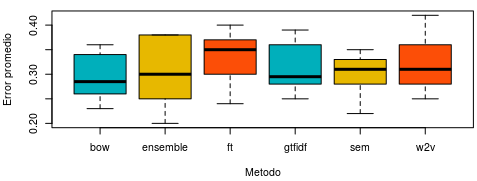
\includegraphics[width=0.7\linewidth]{10_resultados/imagenes/anova_100}
	\caption{Gráfico de caja y bigote para las medias de error de los métodos en estudio para tamaño de muestra de 100 pares de preguntas.}
	\label{fig:anova100}
\end{figure}

\bigskip El método EQuAL posee una media de error que no posee diferencias significativas a todos los métodos. En todos los casos, los intervalos de confianza incluyen al valor 0 y \(p-adj > \alpha\). La Figura \ref{fig:anova100} muestra un gráfico de caja y bigote para las medias de error en estudio y tamaño de muestra 100. En la misma, se puede visualizar que el método EQuAL posee el menor valor de error para una ejecución individual en particular, representado por el bigote inferior.

\bigskip
\paragraph{Tamaño de muestra de 500 pares de preguntas}
\begin{rc}
                  diff          lwr         upr     p adj
ensemble-bow     0.0018 -0.016671384 0.020271384 0.9997181
ft-ensemble      0.0142 -0.004271384 0.032671384 0.2237050
gtfidf-ensemble  0.0078 -0.010671384 0.026271384 0.8113536
sem-ensemble     0.0036 -0.014871384 0.022071384 0.9922183
w2v-ensemble     0.0106 -0.007871384 0.029071384 0.5407045
\end{rc}

\begin{figure}
	\centering
	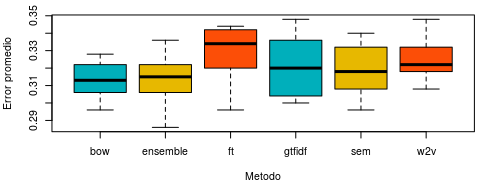
\includegraphics[width=0.7\linewidth]{10_resultados/imagenes/anova_500}
	\caption{Gráfico de caja y bigote para las medias de error de los métodos en estudio para tamaño de muestra de 500 pares de preguntas.}
	\label{fig:anova500}
\end{figure}

\bigskip El método EQuAL posee una media de error que no posee diferencias significativas a todos los métodos. En todos los casos, los intervalos de confianza incluyen al valor 0 y \(p-adj > \alpha\). La Figura \ref{fig:anova500} muestra un gráfico de caja y bigote para las medias de error en estudio y tamaño de muestra 500. En la misma, se puede visualizar que el método EQuAL posee el menor valor de error para una ejecución individual en particular, representado por el bigote inferior.

\bigskip
\paragraph{Tamaño de muestra de 1000 pares de preguntas}
\begin{rc}
                  diff          lwr         upr     p adj
ensemble-bow     0.0175 -0.004161633 0.039161633 0.1791584
ft-ensemble     -0.0049 -0.026561633 0.016761633 0.9846755
gtfidf-ensemble -0.0072 -0.028861633 0.014461633 0.9217004
sem-ensemble    -0.0162 -0.037861633 0.005461633 0.2504112
w2v-ensemble    -0.0155 -0.037161633 0.006161633 0.2956972
\end{rc}

\begin{figure}
	\centering
	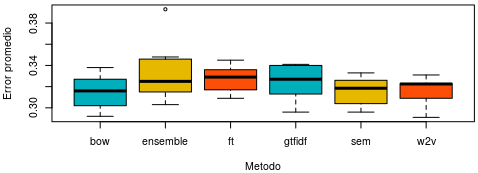
\includegraphics[width=0.7\linewidth]{10_resultados/imagenes/anova_1000}
	\caption{Gráfico de caja y bigote para las medias de error de los métodos en estudio para tamaño de muestra de 1000 pares de preguntas.}
	\label{fig:anova1000}
\end{figure}

\bigskip El método EQuAL posee una media de error que no posee diferencias significativas a todos los métodos. En todos los casos, los intervalos de confianza incluyen al valor 0 y \(p-adj > \alpha\). La Figura \ref{fig:anova1000} muestra un gráfico de caja y bigote para las medias de error en estudio y tamaño de muestra 1000.

\bigskip
\paragraph{Tamaño de muestra de 1500 pares de preguntas}
\begin{rc}
                        diff           lwr         upr     p adj
ensemble-bow     0.0090666667 -7.427521e-03 0.025560854 0.5832109
ft-ensemble      0.0027333333 -1.376085e-02 0.019227521 0.9962642
gtfidf-ensemble  0.0028666667 -1.362752e-02 0.019360854 0.9953275
sem-ensemble     0.0044666667 -1.202752e-02 0.020960854 0.9656207
w2v-ensemble    -0.0062000000 -2.269419e-02 0.010294187 0.8729702
\end{rc}

\begin{figure}
	\centering
	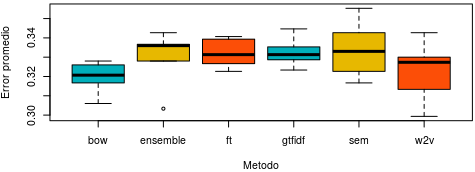
\includegraphics[width=0.7\linewidth]{10_resultados/imagenes/anova_1500}
	\caption{Gráfico de caja y bigote para las medias de error de los métodos en estudio para tamaño de muestra de 1500 pares de preguntas.}
	\label{fig:anova1500}
\end{figure}

\bigskip El método EQuAL posee una media de error que no posee diferencias significativas a todos los métodos. En todos los casos, los intervalos de confianza incluyen al valor 0 y \(p-adj > \alpha\). La Figura \ref{fig:anova1500} muestra un gráfico de caja y bigote para las medias de error en estudio y tamaño de muestra 1500.

\bigskip
\paragraph{Tamaño de muestra de 2000 pares de preguntas}
\begin{rc}
                  diff       lwr       upr      p adj
ensemble-bow     0.01585  0.001648 0.0300516 0.020523
ft-ensemble      0.00385 -0.010351 0.0180516 0.965462
gtfidf-ensemble -0.00035 -0.014551 0.0138516 0.999999
sem-ensemble    -0.00570 -0.019901 0.0085016 0.839375
w2v-ensemble    -0.00725 -0.021451 0.0069516 0.657185
\end{rc}

\begin{figure}
	\centering
	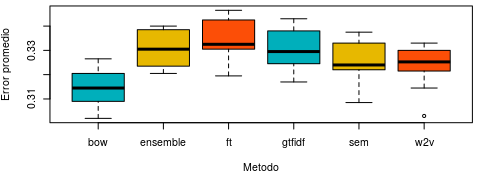
\includegraphics[width=0.7\linewidth]{10_resultados/imagenes/anova_2000}
	\caption{Gráfico de caja y bigote para las medias de error de los métodos en estudio para tamaño de muestra de 2000 pares de preguntas.}
	\label{fig:anova2000}
\end{figure}

\bigskip En este caso, el intervalos de confianza contra el método bow no incluye al cero, ya que este método tuvo muy buenos indicadores en este tamaño de muestra. No obstante, el método EQuAL tiene una diferencia significativa solo con el método bow, no habiendo diferencias significativas con los métodos restantes, ya que en esos casos, los intervalos de confianza incluyen al valor \(0\) y \(p-adj > \alpha\). La Figura \ref{fig:anova2000} muestra un gráfico de caja y bigote para las medias de error en estudio y tamaño de muestra 2000.

\bigskip
\paragraph{Resumen de resultados del análisis de varianza}
En general, el método EQuAL tiene un buen comportamiento en cuanto a medias de error a lo largo de todos los tamaños de muestra. Esto significa que las esperanzas de error no tienen diferencias significativas con los métodos del estado del arte (los cuales son utilizados por la comunidad en el cálculo de similaridad y análisis de texto) y son, incluso, superadoras en algunos casos. Teniendo en cuenta este indicador, se puede concluir que el método EQuAL es apto para su implementación en RSs.

\subsubsection{Desempeño con tamaños de muestra pequeños}
En el análisis de varianza de las medias de error realizado anteriormente, se puede observar que el método EQuAL se comporta muy bien en los tamaños de muestra de 100 y 500 pares de preguntas: el método propuesto fue estadísticamente igual o superior a los métodos del estado del arte. Sin embargo, para tamaños de muestra más grandes, fue superado en algunas oportunidades.

\bigskip Esto demuestra que el agregado de variabilidad de datos puede ser influyente en el cálculo de similaridad. Los métodos del estado del arte cada una de las preguntas de cada para entre sí, mientras que el método EQuAL realiza una comparación “todas contra todas” con el objetivo de realizar un método de clustering a continuación. Para clarificar, se puede concluir que los gráficos y estadísticas obtenidos muestran que métodos basados en ensamble de clustering, y en particular el método EQuAL,  proponen una medida de similaridad adimensional que puede mejorar ciertas medidas de rendimiento en comparativa con otros algoritmos. Citando a \cite{fred2005combining} esta mejora se hace aún más evidente en tamaños de muestras chicos o conjuntos de datos complejos.

\subsubsection{Dependencia de un método de ensamble con sus algoritmos subyacentes}
Si bien es una medida adimensional y propone mejorar las medidas de rendimiento en ciertos aspectos, los métodos de ensamble de clustering son dependientes de sus algoritmos subyacentes y, por lo tanto, las medidas de desempeño son similares en cuanto a, por ejemplo, el valor de error obtenido. Los análisis de varianza realizados ponen en evidencia la dependencia del método equal con los algoritmos ensamblados. La media de error es la misma (estadísticamente hablando) en la mayoría de los casos, lo cual indica que los valores arrojados por el método de ensamble son directamente proporcionales a las medias subyacentes, dando la posibilidad de mejorar los indicadores de rendimiento cuando se utilicen algoritmos de similaridad de texto que tengan mejor comportamiento.

\subsubsection{Influencia del conjunto de datos Quora}
En las secciones anteriores se demostró que el método EQuAL es apto para la utilización en un sistema de recomendación. No obstante, no posee ventajas claras sobre los métodos del estado del arte en algunas medidas de rendimiento en particular.

\bigskip El conjunto de datos Quora y la naturaleza del mismo, no permite realizar un diagrama de dispersión que posibilite ver la forma de los clusters generados. Dicho esto, y sabiendo que la técnica de Ensamble de Clustering es particularmente efectiva en la detección de clusters con formas no convencionales, no es posible identificar fácilmente cuál es la forma de los clusters en cuestión, y verificar si el método EQuAL se adapta perfectamente al conjunto de datos.

\bigskip Por otro lado, el conjunto de datos compara preguntas una a una, que generalmente tienen una o más palabras en común. Esto provoca que los métodos como TF o TFIDF que cuantifican la cantidad de palabras en común, se comporten relativamente bien o arrojen, al menos, un  resultado distinto de cero que supera a los métodos “más inteligentes”. Lo contrario ocurriría, si la comparación de texto fuese entre frases cortas que utilicen sinónimos o palabras completamente distintas, donde los algoritmos basados en taxonomías y técnicas de ML tendrían clara ventaja.

\bigskip El método EQuAL, no es únicamente efectivo para algoritmos subyacentes basados en análisis de texto, sino que también es posible utilizarlo para cualquier conjunto de datos y técnica que generen matrices de distancia como salida. Tal es así, que podría funcionar de manera excepcional con conjuntos de datos que puedan ser graficados y tengan clusters identificables visualmente, con formas que sean convenientes para métodos basados en Ensamble de Clustering.

\subsection{Análisis de desempeño}

El objetivo del análisis de desempeño es evaluar si el mismo es afectado por el paralelismo que otorga Apache Spark. El cluster de prueba consiste en un cluster local, por lo cual el paralelismo será realizado modificando la cantidad de núcleos CPU que se le provee al cluster Hadoop local. Esta configuración puede ser extrapolada fácilmente a un cluster de computadoras con más de un nodo, y con varios ejecutores por nodo.

\bigskip Las pruebas son realizadas ejecutando los experimentos de forma local y variando la configuración del contexto Spark. Ya que en este trabajo, la etapa de clustering no se realizó utilizando Apache Spark, no es detallada en esta sección. Se analizan entonces, la etapa de cálculo de similaridad, el ensamble de clustering y luego la ejecución total de los experimentos, con tamaños de muestra 100, 500 y 1000 pares de preguntas. Cada una de las ejecuciones, se realizan utilizando dos técnicas de similaridad (TF y TFIDF), para luego ensamblarlas. Además, con cada una de ellas, se realizó un algoritmo de clustering con \(k = 5\) y \(20\) ejecuciones del mismo. Las pruebas de rendimiento se realizaron con el siguiente equipo:

\begin{verbatim}
Modelo: MacBook Pro
Procesador: Intel Core i7
Velocidad del procesador: 2.6 GHz
Numero de nucleos: 6
Caché L2 (por núcleo): 256 KB
Caché L3: 12 MB
Tecnología Hyper-Threading: Habilitada
Memoria: 16 GB RAM
Almacenamiento: APPLE SSD AP0512M
\end{verbatim}

\bigskip La cantidad de núcleos de CPU asignados al contexto Spark variará de 1 a 12. La \textbf{Tabla \ref{tab:calc-matrices-sim}} 0 muestra los el tiempo total para la etapa de cálculo de matrices de similaridad, y una estimación de cálculos/segundo siendo la cantidad de cálculos total de \(2n^2-n\) por cada una de las matrices de similaridad generadas (dos en total en las pruebas de desempeño). La \textbf{Tabla \ref{tab:calc-ensamble}} muestra los tiempos para la etapa de ensamble de clustering, y una estimación de cálculos/segundo siendo la cantidad de cálculos total de \(N^2n^2\) siendo \(N\) la cantidad de ejecuciones del algoritmo de clustering en total. Para finalizar, la \textbf{Tabla \ref{tab:calc-total}}  muestra los tiempos totales de cada una de las ejecuciones. El tiempo total está compuesto un tiempo de preprocesamiento, cálculos de similaridades, algoritmos de clustering y ensamble de clustering\footnote{Detalles de los tiempos de ejecución en la tabla X.X.X.}. La cantidad estimada de calculos total, es la sumatoria de los dos explicados anteriormente más una cantidad estimada para las ejecuciones del algoritmo de clustering \(Nnki\), donde \(N=40\) ejecuciones, \(k=5\) clusters para \(i=300\) iteraciones.

\begin{table}[]
	\centering
	\begin{tabular}{|c|c|c|c|c|}
		\hline
		\multicolumn{5}{|c|}{\cellcolor[HTML]{DAE8FC}\textbf{Cálculo de matrices de similaridad}}  \\ \hline
		\cellcolor[HTML]{DAE8FC} &
		\cellcolor[HTML]{DAE8FC} &
		\cellcolor[HTML]{DAE8FC} &
		\cellcolor[HTML]{DAE8FC} &
		\cellcolor[HTML]{DAE8FC} \\
		\multirow{-2}{*}{\cellcolor[HTML]{DAE8FC}\textbf{Núcleo CPU}} &
		\multirow{-2}{*}{\cellcolor[HTML]{DAE8FC}\textbf{Tamaño de muestra}} &
		\multirow{-2}{*}{\cellcolor[HTML]{DAE8FC}\textbf{Cálculos}} &
		\multirow{-2}{*}{\cellcolor[HTML]{DAE8FC}\textbf{Tiempo}} &
		\multirow{-2}{*}{\cellcolor[HTML]{DAE8FC}\textbf{Calc/seg}} \\ \hline
		1  & 100   & 39996   & 62.990                           & 634.957                          \\ \hline
		2  & 100   & 39996   & 46.081                           & 867.955                          \\ \hline
		4  & 100   & 39996   & 33.074                           & 1209.303                         \\ \hline
		8  & 100   & 39996   & 31.276                           & 1278.827                         \\ \hline
		12 & 100   & 39996   & 32.336                           & 1236.882                         \\ \hline
		1  & 500   & 999996  & 763.889                          & 1309.086                         \\ \hline
		2  & 500   & 999996  & 576.669                          & 1734.091                         \\ \hline
		4  & 500   & 999996  & 402.376                          & 2485.226                         \\ \hline
		8  & 500   & 999996  & 324.826                          & 3078.561                         \\ \hline
		12 & 500   & 999996  & 328.300                          & 3045.980                         \\ \hline
		1  & 1,000 & 3999996 & 2950.810                         & 1355.559                         \\ \hline
		2  & 1,000 & 3999996 & 2073.179                         & 1929.402                         \\ \hline
		4  & 1,000 & 3999996 & \multicolumn{1}{r|}{1423.895968} & \multicolumn{1}{r|}{2809.191184} \\ \hline
		8  & 1,000 & 3999996 & \multicolumn{1}{r|}{1176.5926}   & \multicolumn{1}{r|}{3399.644023} \\ \hline
		12 & 1,000 & 3999996 & \multicolumn{1}{r|}{1253.433926} & \multicolumn{1}{r|}{3191.230042} \\ \hline
	\end{tabular}
	\caption{Cálculos aproximados y tiempo para la etapa de cálculo de matrices de similaridad para los distintos tamaños de muestra.}
	\label{tab:calc-matrices-sim}
\end{table}

\begin{table}[]
	\centering
	\begin{tabular}{|c|c|c|c|c|}
		\hline
		\multicolumn{5}{|c|}{\cellcolor[HTML]{DAE8FC}\textbf{Ensamble de Clustering}} \\ \hline
		\cellcolor[HTML]{DAE8FC} &
		\cellcolor[HTML]{DAE8FC} &
		\cellcolor[HTML]{DAE8FC} &
		\cellcolor[HTML]{DAE8FC} &
		\cellcolor[HTML]{DAE8FC} \\
		\multirow{-2}{*}{\cellcolor[HTML]{DAE8FC}\textbf{Núcleo CPU}} &
		\multirow{-2}{*}{\cellcolor[HTML]{DAE8FC}\textbf{Tamaño de muestra}} &
		\multirow{-2}{*}{\cellcolor[HTML]{DAE8FC}\textbf{Cálculos}} &
		\multirow{-2}{*}{\cellcolor[HTML]{DAE8FC}\textbf{Tiempo}} &
		\multirow{-2}{*}{\cellcolor[HTML]{DAE8FC}\textbf{Calc/seg}} \\ \hline
		1        & 100         & 16000000        & 15.978         & 1001359.283       \\ \hline
		2        & 100         & 16000000        & 10.388         & 1540193.812       \\ \hline
		4        & 100         & 16000000        & 6.872          & 2328158.952       \\ \hline
		8        & 100         & 16000000        & 6.309          & 2536184.216       \\ \hline
		12       & 100         & 16000000        & 5.698          & 2808037.305       \\ \hline
		1        & 500         & 400000000       & 40.430         & 9893694.968       \\ \hline
		2        & 500         & 400000000       & 25.684         & 15573735.642      \\ \hline
		4        & 500         & 400000000       & 21.511         & 18594808.023      \\ \hline
		8        & 500         & 400000000       & 18.017         & 22201723.864      \\ \hline
		12       & 500         & 400000000       & 15.737         & 25417188.196      \\ \hline
		1        & 1,000       & 1600000000      & 95.886         & 16686498.744      \\ \hline
		2        & 1,000       & 1600000000      & 58.053         & 27560883.672      \\ \hline
		4        & 1,000       & 1600000000      & 47.732525      & 33520120.71       \\ \hline
		8        & 1,000       & 1600000000      & 43.265526      & 36980944.14       \\ \hline
		12       & 1,000       & 1600000000      & 43.699182      & 36613957.67       \\ \hline
	\end{tabular}
	\caption{Cálculos aproximados y tiempo para la etapa de ensamble de clustering para los distintos tamaños de muestra.}
	\label{tab:calc-ensamble}
\end{table}

\begin{table}[]
	\centering
	\begin{tabular}{|c|c|c|c|c|}
		\hline
		\multicolumn{5}{|c|}{\cellcolor[HTML]{DAE8FC}\textbf{Total}} \\ \hline
		\cellcolor[HTML]{DAE8FC} &
		\cellcolor[HTML]{DAE8FC} &
		\cellcolor[HTML]{DAE8FC} &
		\cellcolor[HTML]{DAE8FC} &
		\cellcolor[HTML]{DAE8FC} \\
		\multirow{-2}{*}{\cellcolor[HTML]{DAE8FC}\textbf{Núcleo CPU}} &
		\multirow{-2}{*}{\cellcolor[HTML]{DAE8FC}\textbf{Tamaño de muestra}} &
		\multirow{-2}{*}{\cellcolor[HTML]{DAE8FC}\textbf{Cálculos}} &
		\multirow{-2}{*}{\cellcolor[HTML]{DAE8FC}\textbf{Tiempo}} &
		\multirow{-2}{*}{\cellcolor[HTML]{DAE8FC}\textbf{Calc/seg}} \\ \hline
		1    & 100     & 40039996     & 88.554        & 452154.152   \\ \hline
		2    & 100     & 40039996     & 64.830        & 617610.886   \\ \hline
		4    & 100     & 40039996     & 47.607        & 841058.532   \\ \hline
		8    & 100     & 40039996     & 45.024        & 889313.092   \\ \hline
		12   & 100     & 40039996     & 44.428        & 901233.021   \\ \hline
		1    & 500     & 520999996    & 828.022       & 629210.531   \\ \hline
		2    & 500     & 520999996    & 624.102       & 834799.734   \\ \hline
		4    & 500     & 520999996    & 446.984       & 1165589.860  \\ \hline
		8    & 500     & 520999996    & 363.617       & 1432826.642  \\ \hline
		12   & 500     & 520999996    & 362.982       & 1435333.416  \\ \hline
		1    & 1,000   & 1843999996   & 3106.846      & 593527.943   \\ \hline
		2    & 1,000   & 1843999996   & 2199.752      & 838276.366   \\ \hline
		4    & 1,000   & 1843999996   & 1530.309932   & 1204984.662  \\ \hline
		8    & 1,000   & 1843999996   & 1282.804328   & 1437475.658  \\ \hline
		12   & 1,000   & 1843999996   & 1370.473092   & 1345520.76   \\ \hline
	\end{tabular}
	\caption{Cálculos aproximados y tiempos totales para los distintos tamaños de muestra.}
	\label{tab:calc-total}
\end{table}

Graficando las tablas \ref{tab:calc-matrices-sim} y \ref{tab:calc-ensamble} para cada uno de los tamaños de muestra de forma sumarizada, se puede ver claramente como el desempeño aumenta hasta cierto nivel de paralelismo. En un cluster Spark, existe una cota superior al número de nodos/ejecutores/CPU en el cual más allá del mismo, el aumento del desempeño es marginal. Este límite depende de la naturaleza de la aplicación y difiere notablemente si la misma hace uso intensivo de CPU o uso intensivo de operaciones de entrada-salida.

\begin{filecontents*}{performance100.csv}
1,62.9900532,15.978281,88.5538612
2,46.080726,10.388303,64.830457
4,33.073601,6.872383,47.60667
8,31.275526,6.30869,45.023509
12,32.336151,5.69793,44.428017
\end{filecontents*}

\begin{figure}
	\centering
	\scriptsize
	\resizebox{\textwidth}{!}{%
		\begin{tikzpicture}
			\begin{axis}[
				xlabel={Número de núcleos de CPU},
				ylabel={Tiempo (Seg.)},
				xmin=0, xmax=13,
				ymin=0, ymax=100,
				xtick={1,2,4,8,12},
				ytick={0,10,...,100},
				legend pos=north west,
				ymajorgrids=true,
				grid style=dashed,
				]

				\addplot table [mark=square,x index=0, y index=1, col sep=comma] {performance100.csv};
				\label{similaridad100}
				\addplot table [mark=square,x index=0, y index=2, col sep=comma] {performance100.csv};
				\label{ensamble100}
				\addplot table [mark=square,x index=0, y index=3, col sep=comma] {performance100.csv};
				\label{total100}
			\end{axis}

			% Cuadro de leyendas.
			\node [draw,fill=white] at (rel axis cs: 0.66,0.85) {\scriptsize\shortstack[l]{
					\ref{similaridad100} Cálculo de Similaridad \\
					\ref{ensamble100} Ensamble de Clustering \\
					\ref{total100} Total}};
		\end{tikzpicture}
	}
	\caption{Tiempos en segundos para ejecuciones de tamaño de muestra de 100 pares de preguntas y distintos núcleos de CPU.}
	\label{fig:performance100}
\end{figure}

\begin{filecontents*}{performance500.csv}
1,763.888817,15.161685,828.022
2,576.668802,15.091077,624.102
4,402.376359,16.416085,446.984
8,324.825807,14.482088,363.617
12,328.300206,12.980533,362.982
\end{filecontents*}

\begin{figure}
	\centering
	\scriptsize
	\resizebox{\textwidth}{!}{%
		\begin{tikzpicture}
			\begin{axis}[
				xlabel={Número de núcleos de CPU},
				ylabel={Tiempo (Seg.)},
				xmin=0, xmax=13,
				ymin=0, ymax=1000,
				xtick={1,2,4,8,12},
				ytick={0,100,...,1000},
				legend pos=north west,
				ymajorgrids=true,
				grid style=dashed,
				]

				\addplot table [mark=square,x index=0, y index=1, col sep=comma] {performance500.csv};
				\label{similaridad500}
				\addplot table [mark=square,x index=0, y index=2, col sep=comma] {performance500.csv};
				\label{ensamble500}
				\addplot table [mark=square,x index=0, y index=3, col sep=comma] {performance500.csv};
				\label{total500}
			\end{axis}

			% Cuadro de leyendas.
			\node [draw,fill=white] at (rel axis cs: 0.66,0.85) {\scriptsize\shortstack[l]{
					\ref{similaridad500} Cálculo de Similaridad \\
					\ref{ensamble500} Ensamble de Clustering \\
					\ref{total500} Total}};
		\end{tikzpicture}
	}
	\caption{Tiempos en segundos para ejecuciones de tamaño de muestra de 500 pares de preguntas y distintos núcleos de CPU.}
	\label{fig:performance500}
\end{figure}

\begin{filecontents*}{performance1000.csv}
1,2950.810,50.678,3106.846134
2,2073.179,61.050,2199.751862
4,1423.896,51.581,1530.309932
8,1176.593,56.610,1282.804328
12,1253.434,66.790,1370.473092
\end{filecontents*}

\begin{figure}
	\centering
	\scriptsize
	\resizebox{\textwidth}{!}{%
		\begin{tikzpicture}
			\begin{axis}[
				xlabel={Número de núcleos de CPU},
				ylabel={Tiempo (Seg.)},
				xmin=0, xmax=13,
				ymin=0, ymax=3500,
				xtick={1,2,4,8,12},
				ytick={0,500,...,3500},
				legend pos=north west,
				ymajorgrids=true,
				grid style=dashed,
				]

				\addplot table [mark=square,x index=0, y index=1, col sep=comma] {performance1000.csv};
				\label{similaridad1000}
				\addplot table [mark=square,x index=0, y index=2, col sep=comma] {performance1000.csv};
				\label{ensamble1000}
				\addplot table [mark=square,x index=0, y index=3, col sep=comma] {performance1000.csv};
				\label{total1000}
			\end{axis}

			% Cuadro de leyendas.
			\node [draw,fill=white] at (rel axis cs: 0.66,0.85) {\scriptsize\shortstack[l]{
					\ref{similaridad1000} Cálculo de Similaridad \\
					\ref{ensamble1000} Ensamble de Clustering \\
					\ref{total1000} Total}};
		\end{tikzpicture}
	}
	\caption{Tiempos en segundos para ejecuciones de tamaño de muestra de 1000 pares de preguntas y distintos núcleos de CPU.}
	\label{fig:performance1000}
\end{figure}

\bigskip El tiempo total de ejecución del método EQuAL decrece exponencialmente configurando un correcto nivel de paralelismo. Por lo cual, la arquitectura propuesta provee un método sencillo para escalar horizontalmente y poder procesar grandes cantidades de datos de forma eficiente. La configuración óptima del cluster de computadoras que soportará la arquitectura depende del tamaño del conjunto de datos de entrada.

\subsection{Resumen de resultados}

En el análisis del método EQuAL, mediante experimentación con distintos parámetros (tamaño de muestra y número de clusters), se obtuvo una media de error mínima de \(0.312\) para el tamaño de muestra de \(100\) pares de preguntas y \(k = 50\). Esta tendencia en los resultados demuestra dos particularidades: el método EQuAL tuvo buen rendimiento con tamaño de muestras chicas y con un alto número de clusters. Esta tendencia en tamaños de muestra chicos puede ser consecuencia del agregado de variabilidad que este método proporciona. Por otro lado, la tendencia a la baja de media de error es mucho más clara con valores de \(k\) altos, obteniendo un valor muy bueno cuando \(k = 50\). Luego de ese valor, la mejora no es significativa.

\bigskip Por otro lado, comparando el método EQuAL con los algoritmos del estado del arte, se concluye que posee indicadores aptos para su aplicación en RSs, en cuanto a medias de error y varianza. La media de error total del método EQuAL (teniendo en cuenta todas las ejecuciones realizadas en los experimentos) es de \(0.32286\), la cual no difiere demasiado de la mejor (bow con \(0.31162\)) y supera a FastText y TFIDF con \(0.33124\) y \(0.32409\) respectivamente.

\bigskip Se realizó un Análisis de Varianza del método propuesto en contraste con los métodos del estado del arte para poder afirmar que el método EQuAL es apto para ser aplicado en RS, de forma eficiente y eficaz, de forma estadísticamente significativa. En la mayoría de los tamaños de muestra analizados, la media de error fue estadísticamente igual en comparación con cada uno de los métodos del estado del arte, con excepción de una oportunidad. En muchas oportunidades el método EQuAL fue superador.

\bigskip Adicionalmente, es posible afirmar que el método propuesto depende tanto de los algoritmos subyacentes como del conjunto de datos de entrada. Por un lado, es altamente probable que arroje buenos resultados si los algoritmos subyacentes también lo hacen, y viceversa. Por otro lado, es posible adaptarlo al conjunto de datos y elegir los algoritmos subyacentes adecuados para el mismo, dando versatilidad y un resultado compuesto por características aportadas por cada uno de ellos.

\bigskip Para finalizar, se desarrolló una arquitectura de software que realiza los cálculos de similaridad y procesamiento del ensamble de clustering de forma distribuida, la cual es escalable horizontalmente permitiendo incrementar el rendimiento de manera exponencial, solo con un cambio de configuración de la infraestructura base.

